% 2018 全国Ⅲ卷文科/理科第9题函数图象选项
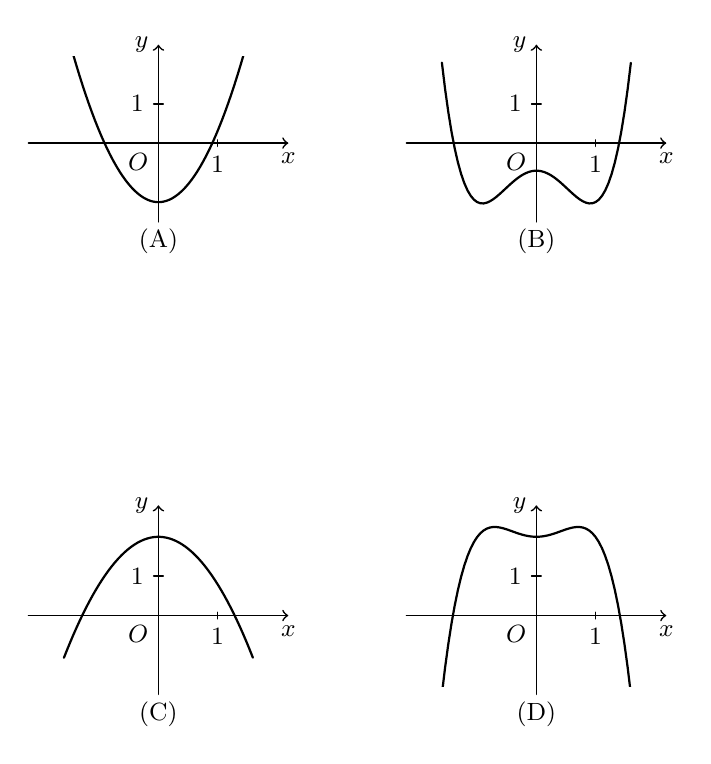
\begin{tikzpicture}[line cap=round, line join=round, line width=0.6pt, font=\small]

% (A) 单峰向上U形
\begin{scope}[shift={(0, 3.2)}, x=0.75cm, y=0.5cm]
  \draw[->] (-2.2, 0) -- (2.2, 0) node[below] {$x$};
  \draw[->] (0, -2.0) -- (0, 2.5) node[left] {$y$};
  \node[below left] at (0, 0) {$O$};
  \draw (1, 0.08) -- (1, -0.08) node[below] {$1$};
  \draw (0.08, 1) -- (-0.08, 1) node[left] {$1$};
  \begin{scope}
    \clip (-2.0, -1.8) rectangle (2.0, 2.2);
    \draw[thick, domain=-1.55:1.55, samples=60] plot (\x, {1.8*(\x)^2 - 1.5});
  \end{scope}
  \node at (0, -2.5) {(A)};
\end{scope}

% (B) 双谷向上W形
\begin{scope}[shift={(4.8, 3.2)}, x=0.75cm, y=0.5cm]
  \draw[->] (-2.2, 0) -- (2.2, 0) node[below] {$x$};
  \draw[->] (0, -2.0) -- (0, 2.5) node[left] {$y$};
  \node[below left] at (0, 0) {$O$};
  \draw (1, 0.08) -- (1, -0.08) node[below] {$1$};
  \draw (0.08, 1) -- (-0.08, 1) node[left] {$1$};
  \begin{scope}
    \clip (-2.0, -1.8) rectangle (2.0, 2.2);
    \draw[thick, domain=-1.6:1.6, samples=60] plot (\x, {1.2*(\x)^4 - 2.0*(\x)^2 - 0.7});
  \end{scope}
  \node at (0, -2.5) {(B)};
\end{scope}

% (C) 单峰向下倒U形
\begin{scope}[shift={(0, -2.8)}, x=0.75cm, y=0.5cm]
  \draw[->] (-2.2, 0) -- (2.2, 0) node[below] {$x$};
  \draw[->] (0, -2.0) -- (0, 2.8) node[left] {$y$};
  \node[below left] at (0, 0) {$O$};
  \draw (1, 0.08) -- (1, -0.08) node[below] {$1$};
  \draw (0.08, 1) -- (-0.08, 1) node[left] {$1$};
  \begin{scope}
    \clip (-2.0, -1.8) rectangle (2.0, 2.5);
    \draw[thick, domain=-1.6:1.6, samples=60] plot (\x, {-1.2*(\x)^2 + 2.0});
  \end{scope}
  \node at (0, -2.5) {(C)};
\end{scope}

% (D) 双峰向下M形（正确选项 y = -x^4 + x^2 + 2）
\begin{scope}[shift={(4.8, -2.8)}, x=0.75cm, y=0.5cm]
  \draw[->] (-2.2, 0) -- (2.2, 0) node[below] {$x$};
  \draw[->] (0, -2.0) -- (0, 2.8) node[left] {$y$};
  \node[below left] at (0, 0) {$O$};
  \draw (1, 0.08) -- (1, -0.08) node[below] {$1$};
  \draw (0.08, 1) -- (-0.08, 1) node[left] {$1$};
  \begin{scope}
    \clip (-2.0, -1.8) rectangle (2.0, 2.5);
    \draw[thick, domain=-1.6:1.6, samples=60] plot (\x, {-(\x)^4 + (\x)^2 + 2.0});
  \end{scope}
  \node at (0, -2.5) {(D)};
\end{scope}

\end{tikzpicture}
